%!TEX root = ../paper.tex
\chapter{ARM平台---树莓派}
	\section{简介}
		\par 树莓派(英语:Raspberry Pi),是一款基于Linux的单板机电脑。它由英国的树莓派基金会所开发,目的是以低价硬件及自由软件促进学校的基本计算机科学教育。
		\par 树莓派的生产是通过有生产许可的两家公司:Element 14/Premier Farnell和RS Components。这两家公司都在网上出售树莓派。
		\par 树莓派配备一枚博通(Broadcom)出产的ARM架构700MHz BCM2835处理器,256MB內存(B型已升级到512MB内存),使用SD卡当作存储媒体,且拥有一个Ethernet、两个USB接口、以及HDMI(支持声音输出)和RCA端子输出支持。树莓派只有一张信用卡大小,体积大概是一个火柴盒大小,可以运行像《雷神之锤III竞技场》的游戏和进行1080p视频的播放。操作系统采用开源的Linux系统如Debian、ArchLinux,自带的Iceweasel、KOffice等软件,能够满足基本的网络浏览、文字处理以及电脑学习的需要。分A、B两种型号,售价分别是A型25美元、B型35美元。树莓派基金会从2012年2月29日开始接受B型的订货。
		\par 树莓派基金会提供了基于ARM架构的Debian、Arch Linux和Fedora等的发行版供大众下载,还计划提供支持Python作为主要编程语言,支持BBC BASIC、C语言和Perl等编程语言。
		树莓派基金会于2016年2月发布了树莓派3,较前一代树莓派2,树莓派3的处理器升级为了64位的博通BCM2837,并首次加入了Wi-Fi无线网络及蓝牙功能,而售价仍然是35美元,表\ref{table:params_of_raspi}为树莓派3B+的参数。\cite{ wiki:树莓派}
		\begin{table}[!ht]
			\centering
			\caption{树莓派3B+参数}
			\begin{tabular}{l|p{0.8\columnwidth}}
				\hline\hline
				SoC          & Broadcom\ BCM2837(CPU,GPU\ DSP和SDRAM、USB)                                       \\
				\hline
				CPU          & ARM\ Cortex-A53\ 64位\ (ARMv8系列)\ 1.2GHz\ (四核心)                                \\
				\hline
				GPU          & Broadcom\ VideoCore\ IV[43],\ OpenGL\ ES\ 2.0,1080p\ 30\ h.264/MPEG-4\ AVC高清解码器 \\
				\hline
				RAM          & 1024\ MB\ (LPDDR2)                                                                        \\
				\hline
				外设       & 14个GPIO及HAT规格铺设                                                               \\
				\hline
				额定功率 & 4.0\ 瓦\ (5V/800mA)                                                                      \\
				\hline
				电源输入 & 5V\ 电压\ (通过MicroUSB或经GPIO输入)                                              \\
				\hline
				总体尺寸 & 85.60\ ×\ 53.98\ 毫米(3.370\ ×\ 2.125\ 英寸)                                    \\
				\hline
				重量       & 45\ g(1.6\ oz)                                                                        \\
				\hline\hline
			\end{tabular}
			\label{table:params_of_raspi}
		\end{table}
	\section{烧录系统镜像}
		\par $\bullet$ Windows
		% \paragraph{Windows}
		\par 首先从官网下载镜像(\href{https://www.raspberrypi.org/downloads/}{https://www.raspberrypi.org/downloads/}),下载完成以后会解压出后缀名为img的镜像文件,使用Win32 Disk Imager(\href{https://sourceforge.net/projects/win32diskimager/files/latest/download}{https://sourceforge.net/projects/win32diskimager/files/latest/download})软件将镜像烧写进SD卡,如图\ref{fig:win32diskimager}。
		\begin{figure}[htp]
			\centering
			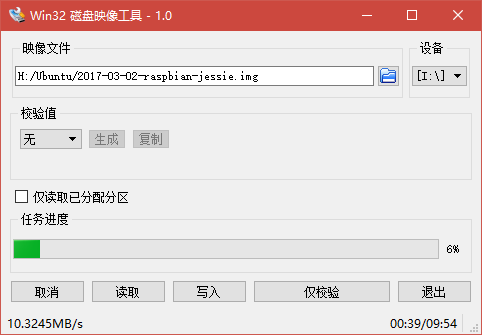
\includegraphics[width=13cm]{figures/win32diskimager.png}
			\caption{Win32DiskImager}
			\label{fig:win32diskimager}
		\end{figure}
		\par $\bullet$ Ubuntu
		\par Ubuntu下使用dd命令进行镜像烧写,首先执行
		\begin{lstlisting}[ language= sh ]
sudo fdisk -l
		\end{lstlisting}
		\par 确认SD卡是否已经挂载,确认已经挂载以后进入镜像文件所在目录执行
		\begin{lstlisting}[ language= sh ]
sudo dd if=2017-03-18-raspbian-jessie-lite.img of=/dev/mmcblk0
		\end{lstlisting}
		\par 稍等片刻即可烧写完成。
		\par 2016.11之前的镜像已经默认开启了ssh登陆,插上卡以后插上网线就能够通过ssh登陆(Windows下使用putty或者xshell,Ubuntu下直接在Terminal下执行\lstinline[language=sh]{ssh pi@192.168.199.1}登陆,\lstinline[language=sh]{@}后为树莓派的ip)。
		\par 2016.11之后的镜像默认关闭了ssh登陆,如需使用ssh登陆,则需要在烧写完成以后,SD卡会分为两个分区,于其中boot目录下新建一个ssh的空白文件(Windows下可以新建文本文件以后删去txt的后缀名,Ubuntu下直接\lstinline[language=sh]{touch ssh}即可)。
		\par 树莓派的系统制作完成以后执行
		\begin{lstlisting}[ language= sh ]
sudo raspi-config
		\end{lstlisting}
		\par 会出现如图\ref{fig:raspi_config}所示界面:
		\begin{figure}[htp]
			\centering
			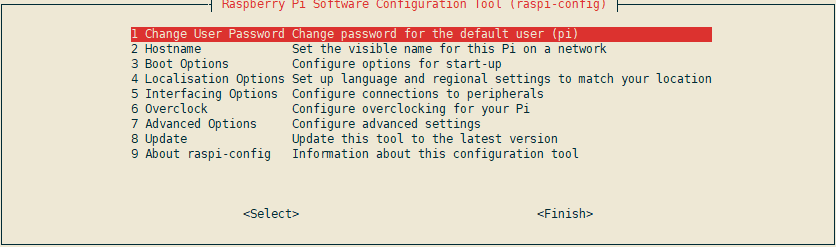
\includegraphics[width=13cm]{figures/raspi-config.png}
			\caption{树莓派配置}
			\label{fig:raspi_config}
		\end{figure}
		\par 其中第一项可以修改用户密码,我们选择\lstinline{Advanced Options}来将系统空间扩展至整个SD卡。
		\begin{figure}[htp]
			\centering
			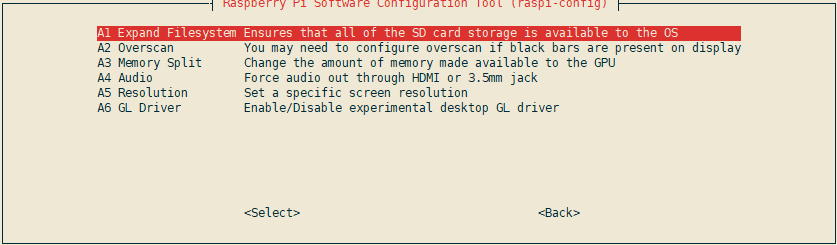
\includegraphics[width=13cm]{figures/raspi-config-expand-filesystem.png}
			\caption{扩展系统空间}
			\label{fig:raspi_config_expand_filesystem}
		\end{figure}
		\par 之后重启系统即可
		\begin{lstlisting}[ language= sh ]
sudo reboot
		\end{lstlisting}
	\section{软件源}
		\par 树莓派默认使用的官方源服务器国内访问不便,国内使用需要使用镜像站,修改\lstinline[language=sh]{/etc/apt/sources.list}为以下内容:
		\begin{lstlisting}[ language= sh ]
deb http://mirrors.ustc.edu.cn/raspbian/raspbian/ jessie main non-free contrib 
deb-src http://mirrors.ustc.edu.cn/raspbian/raspbian/ jessie main non-free contrib
		\end{lstlisting}
		\par 执行
		\begin{lstlisting}[ language= sh ]
sudo apt update
sudo apt upgrade
		\end{lstlisting}
		\par 更新软件,以及各种依赖。
	\section{无线网络配置}
		\par 如果需要将树莓派通过WiFi连接进局域网,则需要配置其无线网络参数,修改\lstinline[language=sh]{/etc/wpa_supplicant/wpa_supplicant.conf}内容为以下内容。
		\begin{lstlisting}
ctrl_interface=DIR=/var/run/wpa_supplicant GROUP=netdev
update_config=1
country=GB

network={
	ssid="your wifi ssid"
	psk="your wifi password"
	priority=5
}
		\end{lstlisting}
		\par 其中:
		\par \lstinline{ssid}为wifi名称。
		\par \lstinline{psk}为wifi密码。
		\par \lstinline{priority}为优先级,数值越大,优先级越高。
		\par 树莓派安装GNU Radio参见\ref{sec:gnuradio}节。
		\par 至此,树莓派的已经基本配置完成。
		% \subsection{镜像备份}
